% Appendix section: fixed-effects specification and inference for the
% regional density regressions. Table and figure are produced by
% scripts/regional/R02_fixed_effects_robustness.py:
%   results/paper/appendix/fe_robustness.tex
%   results/paper/appendix/fe_robustness_annual.png
% Numbers quoted below are from
%   results/regional_fe_robustness/shared_cosine_v16_fe_robustness_period.csv

\section{Fixed-effects specification and inference}
\label{app:fe_robustness}

\paragraph{Main specification.} The regional regressions relate an industry's
entry, exit or startup formation in a municipality to its relatedness density
in a linear probability model,
\begin{equation}
  y_{jmt} = \beta\, \tilde{D}_{jmt} + \alpha_{mt} + \gamma_{j} + \varepsilon_{jmt},
\end{equation}
where $\tilde{D}_{jmt}$ is density $D^{\mathrm{A,log}}$ standardised by its
pooled standard deviation, $\alpha_{mt}$ are municipality$\times$year and
$\gamma_j$ industry fixed effects. The municipality$\times$year effects absorb
everything that varies at the level of a municipality in a given year, such
as total employment, the number of active industries and the local business
cycle, so $\beta$ is identified from differences in density across
industries within the same municipality and year. Because the candidate sets
are unbalanced (entry and startup formation are defined for industries absent
from a municipality in the base year, exit for industries present), the
fixed effects are absorbed exactly by alternating projections iterated to
convergence, after dropping singleton observations. Each model is estimated
separately for the SNI92, SNI02 and SNI07 periods, because code strings
overlap across classification versions but denote different industries.
Year-specific effects are estimated in the same model by interacting density
with base-year indicators.

\paragraph{Inference.} Density is computed from each industry's position in
the latent space and is therefore correlated across municipalities for the
same industry. Standard errors are clustered two-way by municipality and
industry \citep{cameron2011robust}, and confidence intervals and $p$-values
use a $t$ distribution with $\min(G_{\text{municipality}},
G_{\text{industry}})-1$ (288--289) degrees of freedom. With between 0.24 and 1.27
million observations per period, $p$-values are not informative about the
size of the effects; we report $p<0.001$ as a bound and rely on confidence
intervals.

\paragraph{Alternative specifications.} Table~\ref{tab:fe_robustness}
compares the main specification with (2) additive municipality, year and
industry fixed effects and (3) municipality$\times$industry and year fixed
effects, using the same estimator and clustering.
Figure~\ref{fig:fe_robustness_annual} shows the year-specific effects with
95\% confidence intervals.

The additive specification gives estimates close to the main specification
in all periods except SNI92, where the entry and startup formation effects are
somewhat smaller (4.58 vs.\ 6.05 and 0.87 vs.\ 1.05 percentage points), with
overlapping confidence intervals. Municipality--year shocks therefore matter
little beyond additive municipality and year effects.

Specification (3) identifies $\beta$ only from changes in density over time
within a municipality--industry cell. This is a demanding test: most of the
variation in density is between cells, and a cell leaves the candidate set
after an entry (exit) event. In SNI92 and SNI07 the effects keep their signs
and remain significant. For SNI07, the entry and startup formation effects are
larger than in the main specification (6.51 and 3.33 percentage points) and
the exit effect is smaller in magnitude ($-8.91$); for SNI92 all three are
smaller (entry 2.51, exit $-3.68$, startup formation 0.52). In the SNI02 period, which
covers only four base years, the within-cell variation is too small to
estimate the effects precisely, and the confidence intervals include zero
for all three outcomes. Year-specific effects are not shown for this
specification: only their common level is identified from within-cell
changes, while differences between years also draw on cross-sectional
variation, so they are not comparable to the period estimate. The figure
therefore shows its period estimates.

\begin{table}[htbp]
\centering
\small
\caption{Regional density effects under alternative fixed-effects specifications. Each cell reports the coefficient (percentage points per standard deviation of density $D^{\mathrm{A,log}}$) from a linear probability model estimated per classification period, with 95\% confidence intervals in brackets. Fixed effects are absorbed exactly; standard errors are clustered by municipality and industry, and intervals use a $t$ distribution with $\min(G_{\text{municipality}}, G_{\text{industry}})-1$ degrees of freedom. Column 1 is the main specification.}
\label{tab:fe_robustness}
\begin{tabular}{llccc}
\toprule
 & & (1) & (2) & (3) \\
Outcome & Period & Muni$\times$year + industry & Muni + year + industry & Muni$\times$industry + year \\
\midrule
\multirow{3}{*}{Entry} & SNI92 & $\mathbf{6.04}$ [4.44, 7.63] & $4.50$ [2.17, 6.84] & $2.51$ [0.85, 4.17] \\
 & SNI02 & $\mathbf{6.18}$ [3.94, 8.42] & $6.14$ [3.90, 8.38] & $-2.72$ [-9.33, 3.89] \\
 & SNI07 & $\mathbf{5.31}$ [3.53, 7.08] & $5.32$ [3.54, 7.09] & $6.44$ [3.49, 9.39] \\
\addlinespace
\multirow{3}{*}{Exit} & SNI92 & $\mathbf{-13.70}$ [-15.77, -11.63] & $-13.58$ [-15.62, -11.54] & $-3.74$ [-6.70, -0.78] \\
 & SNI02 & $\mathbf{-8.87}$ [-10.40, -7.33] & $-8.92$ [-10.46, -7.39] & $-3.96$ [-9.09, 1.16] \\
 & SNI07 & $\mathbf{-11.78}$ [-13.42, -10.14] & $-11.71$ [-13.35, -10.08] & $-8.94$ [-11.56, -6.31] \\
\addlinespace
\multirow{3}{*}{Startup formation} & SNI92 & $\mathbf{1.05}$ [0.82, 1.29] & $0.87$ [0.59, 1.15] & $0.52$ [0.27, 0.77] \\
 & SNI02 & $\mathbf{1.17}$ [0.54, 1.80] & $1.16$ [0.53, 1.79] & $-0.88$ [-2.92, 1.16] \\
 & SNI07 & $\mathbf{1.72}$ [1.14, 2.30] & $1.73$ [1.14, 2.31] & $3.33$ [2.20, 4.45] \\
\midrule
\multicolumn{2}{l}{Observations (all models)} & 6\,955\,867 & 6\,955\,867 & 6\,905\,186 \\
\bottomrule
\end{tabular}
\end{table}


\begin{figure}[htbp]
  \centering
  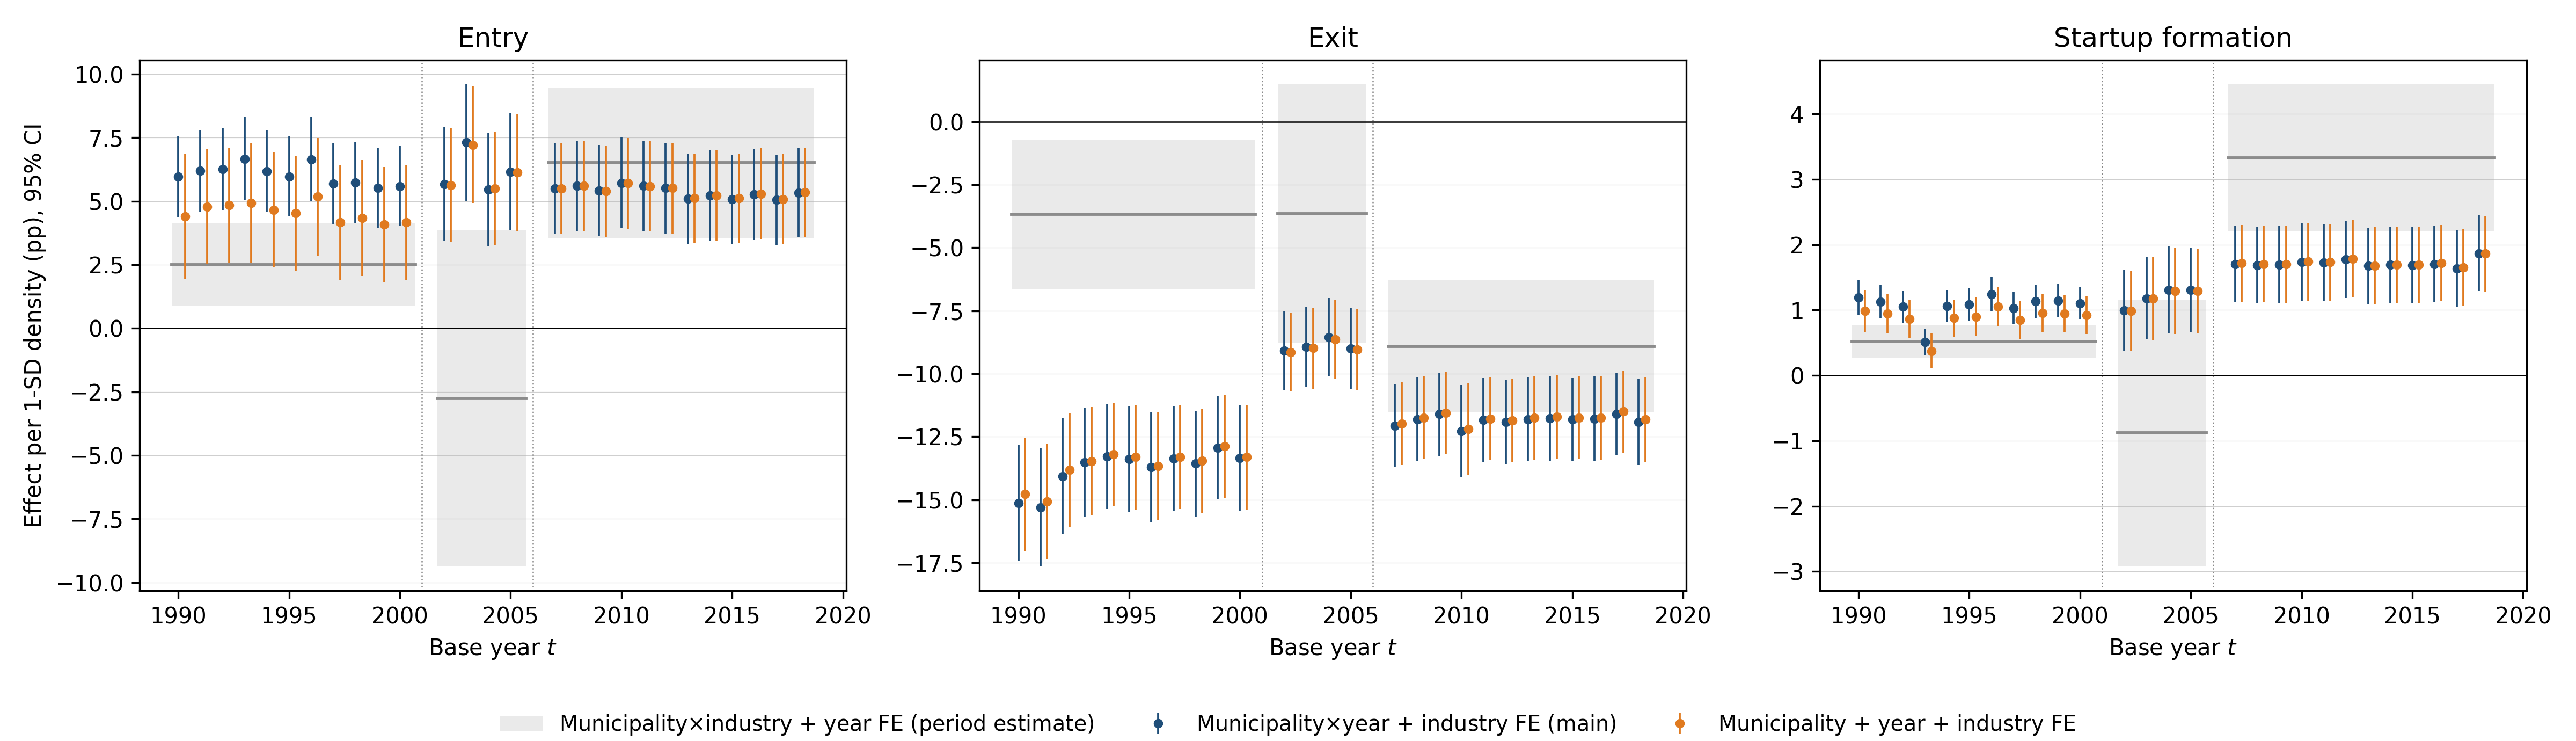
\includegraphics[width=\textwidth]{appendix/fe_robustness_annual.png}
  \caption{Year-specific effects of relatedness density (percentage points
  per standard deviation, 95\% confidence intervals) under the main
  specification (municipality$\times$year and industry fixed effects) and with
  additive municipality, year and industry fixed effects. Grey bands: period
  estimate and 95\% confidence interval with municipality$\times$industry and
  year fixed effects. Standard errors clustered by municipality and industry.
  Dotted lines separate the SNI92, SNI02 and SNI07 periods.}
  \label{fig:fe_robustness_annual}
\end{figure}

% BibTeX entry for the clustering reference:
% @article{cameron2011robust,
%   title   = {Robust Inference With Multiway Clustering},
%   author  = {Cameron, A. Colin and Gelbach, Jonah B. and Miller, Douglas L.},
%   journal = {Journal of Business \& Economic Statistics},
%   volume  = {29}, number = {2}, pages = {238--249}, year = {2011}
% }
